\documentclass{article}\usepackage[]{graphicx}\usepackage[]{color}
%% maxwidth is the original width if it is less than linewidth
%% otherwise use linewidth (to make sure the graphics do not exceed the margin)
\makeatletter
\def\maxwidth{ %
  \ifdim\Gin@nat@width>\linewidth
    \linewidth
  \else
    \Gin@nat@width
  \fi
}
\makeatother

\definecolor{fgcolor}{rgb}{0.345, 0.345, 0.345}
\newcommand{\hlnum}[1]{\textcolor[rgb]{0.686,0.059,0.569}{#1}}%
\newcommand{\hlstr}[1]{\textcolor[rgb]{0.192,0.494,0.8}{#1}}%
\newcommand{\hlcom}[1]{\textcolor[rgb]{0.678,0.584,0.686}{\textit{#1}}}%
\newcommand{\hlopt}[1]{\textcolor[rgb]{0,0,0}{#1}}%
\newcommand{\hlstd}[1]{\textcolor[rgb]{0.345,0.345,0.345}{#1}}%
\newcommand{\hlkwa}[1]{\textcolor[rgb]{0.161,0.373,0.58}{\textbf{#1}}}%
\newcommand{\hlkwb}[1]{\textcolor[rgb]{0.69,0.353,0.396}{#1}}%
\newcommand{\hlkwc}[1]{\textcolor[rgb]{0.333,0.667,0.333}{#1}}%
\newcommand{\hlkwd}[1]{\textcolor[rgb]{0.737,0.353,0.396}{\textbf{#1}}}%
\let\hlipl\hlkwb

\usepackage{framed}
\makeatletter
\newenvironment{kframe}{%
 \def\at@end@of@kframe{}%
 \ifinner\ifhmode%
  \def\at@end@of@kframe{\end{minipage}}%
  \begin{minipage}{\columnwidth}%
 \fi\fi%
 \def\FrameCommand##1{\hskip\@totalleftmargin \hskip-\fboxsep
 \colorbox{shadecolor}{##1}\hskip-\fboxsep
     % There is no \\@totalrightmargin, so:
     \hskip-\linewidth \hskip-\@totalleftmargin \hskip\columnwidth}%
 \MakeFramed {\advance\hsize-\width
   \@totalleftmargin\z@ \linewidth\hsize
   \@setminipage}}%
 {\par\unskip\endMakeFramed%
 \at@end@of@kframe}
\makeatother

\definecolor{shadecolor}{rgb}{.97, .97, .97}
\definecolor{messagecolor}{rgb}{0, 0, 0}
\definecolor{warningcolor}{rgb}{1, 0, 1}
\definecolor{errorcolor}{rgb}{1, 0, 0}
\newenvironment{knitrout}{}{} % an empty environment to be redefined in TeX

\usepackage{alltt}
\usepackage[sc]{mathpazo}
\renewcommand{\sfdefault}{lmss}
\renewcommand{\ttdefault}{lmtt}
\usepackage[T1]{fontenc}
\usepackage{geometry}
\geometry{verbose,tmargin=2.5cm,bmargin=2.5cm,lmargin=2.5cm,rmargin=2.5cm}
\setcounter{secnumdepth}{2}
\setcounter{tocdepth}{2}
\usepackage[unicode=true,pdfusetitle,
 bookmarks=true,bookmarksnumbered=true,bookmarksopen=true,bookmarksopenlevel=2,
 breaklinks=false,pdfborder={0 0 1},backref=false,colorlinks=false]
 {hyperref}
\hypersetup{
 pdfstartview={XYZ null null 1}}

\makeatletter
%%%%%%%%%%%%%%%%%%%%%%%%%%%%%% User specified LaTeX commands.
\renewcommand{\textfraction}{0.05}
\renewcommand{\topfraction}{0.8}
\renewcommand{\bottomfraction}{0.8}
\renewcommand{\floatpagefraction}{0.75}

\makeatother
\IfFileExists{upquote.sty}{\usepackage{upquote}}{}
\begin{document}








The results below are generated from an R script.

\begin{knitrout}
\definecolor{shadecolor}{rgb}{0.969, 0.969, 0.969}\color{fgcolor}\begin{kframe}
\begin{alltt}
\hlcom{## November 2017, Alice Balard}
\hlkwd{library}\hlstd{(ggplot2)}
\hlkwd{library}\hlstd{(ggmap)}
\hlkwd{library}\hlstd{(data.table)}

\hlkwd{source}\hlstd{(}\hlstr{"HMHZ_Functions.R"}\hlstd{)}

\hlstd{MiceTable} \hlkwb{<-} \hlkwd{read.csv}\hlstd{(}\hlstr{"../raw_data/MiceTable_2014to2017.csv"}\hlstd{)}
\hlstd{TrapTable} \hlkwb{<-} \hlkwd{read.csv}\hlstd{(}\hlstr{"../raw_data/TrapTable_2014to2017.csv"}\hlstd{)}

\hlcom{## Remove the Poland data}
\hlstd{MiceTable} \hlkwb{<-} \hlstd{MiceTable[}\hlkwd{which}\hlstd{(MiceTable}\hlopt{$}\hlstd{Longitude} \hlopt{<} \hlnum{17}\hlstd{),]}

\hlcom{## Remove the non Mus musculus (until further notice)}
\hlstd{MiceTable}\hlopt{$}\hlstd{Species[}\hlkwd{is.na}\hlstd{(MiceTable}\hlopt{$}\hlstd{Species)]} \hlkwb{<-} \hlstr{"Mus musculus"}

\hlstd{MiceTable} \hlkwb{<-} \hlstd{MiceTable[}\hlkwd{which}\hlstd{(MiceTable}\hlopt{$}\hlstd{Species} \hlopt{==} \hlstr{"Mus musculus"}\hlstd{),]}

\hlcom{# Check calculation of ALL HI}
\hlstd{markers} \hlkwb{<-} \hlkwd{c}\hlstd{(}\hlstr{"mtBamH"}\hlstd{,} \hlstr{"Zfy2"}\hlstd{,} \hlstr{"SRY1"}\hlstd{,} \hlstr{"Y"}\hlstd{,} \hlstr{"X332"}\hlstd{,} \hlstr{"X347"}\hlstd{,} \hlstr{"X65"}\hlstd{,} \hlstr{"Tsx"}\hlstd{,} \hlstr{"Btk"}\hlstd{,}
             \hlstr{"Syap1"}\hlstd{,} \hlstr{"Es1C"}\hlstd{,} \hlstr{"Gpd1C"}\hlstd{,} \hlstr{"Idh1C"}\hlstd{,} \hlstr{"MpiC"}\hlstd{,} \hlstr{"NpC"}\hlstd{,} \hlstr{"Sod1C"}\hlstd{)}

\hlstd{MiceTable} \hlkwb{<-} \hlkwd{get.HI.full}\hlstd{(}\hlkwc{df} \hlstd{= MiceTable,} \hlkwc{markers.col} \hlstd{= markers)}

\hlcom{# to bear in mind : jarda seems to have calculated HI on different sets of markers}
\hlkwd{table}\hlstd{(MiceTable}\hlopt{$}\hlstd{HI} \hlopt{==} \hlstd{MiceTable}\hlopt{$}\hlstd{HI.calculated)}
\end{alltt}
\begin{verbatim}
## 
## FALSE  TRUE 
##   399   286
\end{verbatim}
\begin{alltt}
\hlcom{# HI per locality}
\hlstd{agglocHI} \hlkwb{<-} \hlkwd{aggregate}\hlstd{(}\hlkwc{x} \hlstd{= MiceTable[}\hlkwd{c}\hlstd{(}\hlstr{"collapsed.GT"}\hlstd{)],}
          \hlkwc{by} \hlstd{= MiceTable[}\hlkwd{c}\hlstd{(}\hlstr{"Latitude"}\hlstd{,} \hlstr{"Longitude"}\hlstd{)],} \hlkwc{FUN} \hlstd{= paste,} \hlkwc{sep} \hlstd{=} \hlstr{"/"} \hlstd{)}

\hlstd{agglocHI}\hlopt{$}\hlstd{HI} \hlkwb{<-} \hlkwd{get.HI}\hlstd{(agglocHI}\hlopt{$}\hlstd{collapsed.GT)}

\hlcom{# ***************************************************************}
\hlcom{## Cluster localities : how many times each LOCALITY was sampled?}

\hlcom{# pairsloc <- pairwise.cluster.loc(trapsTOT) # errors with this model, to discuss}
\hlcom{# loctime <- data.frame(table(apply(pairsloc, 2, sum)))}
\hlcom{# loctime$Var1 <- as.numeric(as.character(loctime$Var1)) + 1 }
\hlcom{# names(loctime) <- c("Repeatition over the years", "# localities")}

\hlkwd{measure}\hlstd{(}\hlkwc{lon1} \hlstd{=} \hlnum{13.04390}\hlstd{,} \hlkwc{lat1} \hlstd{=} \hlnum{51.93000}\hlstd{,} \hlkwc{lon2} \hlstd{=} \hlnum{13.64000}\hlstd{,} \hlkwc{lat2} \hlstd{=} \hlnum{52.71690}\hlstd{)} \hlopt{-} \hlkwd{measure}\hlstd{(}\hlkwc{lon1} \hlstd{=} \hlnum{13.04}\hlstd{,} \hlkwc{lat1} \hlstd{=} \hlnum{51.93}\hlstd{,} \hlkwc{lon2} \hlstd{=} \hlnum{13.64}\hlstd{,} \hlkwc{lat2} \hlstd{=} \hlnum{52.72}\hlstd{)}
\end{alltt}
\begin{verbatim}
## [1] -424.0725
\end{verbatim}
\begin{alltt}
\hlkwd{measure}\hlstd{(}\hlkwc{lon1} \hlstd{=} \hlnum{13.6761}\hlstd{,} \hlkwc{lat1} \hlstd{=} \hlnum{52.4978}\hlstd{,} \hlkwc{lon2} \hlstd{=} \hlnum{13.68}\hlstd{,} \hlkwc{lat2} \hlstd{=} \hlnum{52.50}\hlstd{)}
\end{alltt}
\begin{verbatim}
## [1] 360.3205
\end{verbatim}
\begin{alltt}
\hlcom{# rounded to about 700 meters}
\hlstd{TrapTable}\hlopt{$}\hlstd{Longitude} \hlkwb{<-} \hlkwd{round}\hlstd{(TrapTable}\hlopt{$}\hlstd{Longitude,} \hlnum{2}\hlstd{)}
\hlstd{TrapTable}\hlopt{$}\hlstd{Latitude} \hlkwb{<-} \hlkwd{round}\hlstd{(TrapTable}\hlopt{$}\hlstd{Latitude,} \hlnum{2}\hlstd{)}
\hlstd{MiceTable}\hlopt{$}\hlstd{Latitude} \hlkwb{<-} \hlkwd{round}\hlstd{(MiceTable}\hlopt{$}\hlstd{Latitude,} \hlnum{2}\hlstd{)}
\hlstd{MiceTable}\hlopt{$}\hlstd{Longitude} \hlkwb{<-} \hlkwd{round}\hlstd{(MiceTable}\hlopt{$}\hlstd{Longitude,} \hlnum{2}\hlstd{)}
\hlcom{# ***************************************************************}

\hlcom{# Map}
\hlkwd{HI.map}\hlstd{(agglocHI,} \hlkwc{size} \hlstd{=} \hlnum{4}\hlstd{,} \hlkwc{alpha} \hlstd{=} \hlnum{1}\hlstd{,} \hlkwc{margin} \hlstd{=} \hlnum{0.2}\hlstd{,}\hlkwc{zoom} \hlstd{=} \hlnum{7}\hlstd{)}
\end{alltt}


{\ttfamily\noindent\itshape\color{messagecolor}{\#\# Map from URL : http://tile.stamen.com/toner-lite/7/67/40.png}}

{\ttfamily\noindent\color{warningcolor}{\#\# Warning in file.remove(index[[url]]): cannot remove file 'a6b3537e448e7024d4a3f1fb38927519.rds', reason 'No such file or directory'}}

{\ttfamily\noindent\itshape\color{messagecolor}{\#\# Map from URL : http://tile.stamen.com/toner-lite/7/68/40.png}}

{\ttfamily\noindent\color{warningcolor}{\#\# Warning in file.remove(index[[url]]): cannot remove file '2fc5ddc67ed9d76ebce8634c724afc05.rds', reason 'No such file or directory'}}

{\ttfamily\noindent\itshape\color{messagecolor}{\#\# Map from URL : http://tile.stamen.com/toner-lite/7/69/40.png}}

{\ttfamily\noindent\color{warningcolor}{\#\# Warning in file.remove(index[[url]]): cannot remove file 'aed59ce9a2f30b315a07925a45dd12a9.rds', reason 'No such file or directory'}}

{\ttfamily\noindent\itshape\color{messagecolor}{\#\# Map from URL : http://tile.stamen.com/toner-lite/7/67/41.png}}

{\ttfamily\noindent\color{warningcolor}{\#\# Warning in file.remove(index[[url]]): cannot remove file '839babab850b65c391cabaf8b4f36cc7.rds', reason 'No such file or directory'}}

{\ttfamily\noindent\itshape\color{messagecolor}{\#\# Map from URL : http://tile.stamen.com/toner-lite/7/68/41.png}}

{\ttfamily\noindent\color{warningcolor}{\#\# Warning in file.remove(index[[url]]): cannot remove file 'e2c3be7a0f50f6813780904b3d2b6840.rds', reason 'No such file or directory'}}

{\ttfamily\noindent\itshape\color{messagecolor}{\#\# Map from URL : http://tile.stamen.com/toner-lite/7/69/41.png}}

{\ttfamily\noindent\color{warningcolor}{\#\# Warning in file.remove(index[[url]]): cannot remove file 'e930417ae23f228511270941f5fec9d3.rds', reason 'No such file or directory'}}

{\ttfamily\noindent\itshape\color{messagecolor}{\#\# Map from URL : http://tile.stamen.com/toner-lite/7/67/42.png}}

{\ttfamily\noindent\color{warningcolor}{\#\# Warning in file.remove(index[[url]]): cannot remove file '982a63a7622305a44a475d47314d08ce.rds', reason 'No such file or directory'}}

{\ttfamily\noindent\itshape\color{messagecolor}{\#\# Map from URL : http://tile.stamen.com/toner-lite/7/68/42.png}}

{\ttfamily\noindent\color{warningcolor}{\#\# Warning in file.remove(index[[url]]): cannot remove file 'b92e0b10b3f3c6c59c60d0c83d663135.rds', reason 'No such file or directory'}}

{\ttfamily\noindent\itshape\color{messagecolor}{\#\# Map from URL : http://tile.stamen.com/toner-lite/7/69/42.png}}

{\ttfamily\noindent\color{warningcolor}{\#\# Warning in file.remove(index[[url]]): cannot remove file '258161531a6435b81f700333c8ed105e.rds', reason 'No such file or directory'}}

{\ttfamily\noindent\itshape\color{messagecolor}{\#\# Map from URL : http://tile.stamen.com/toner-lite/7/67/43.png}}

{\ttfamily\noindent\color{warningcolor}{\#\# Warning in file.remove(index[[url]]): cannot remove file 'b65259eba5db3657b783b4cb7f8512b1.rds', reason 'No such file or directory'}}

{\ttfamily\noindent\itshape\color{messagecolor}{\#\# Map from URL : http://tile.stamen.com/toner-lite/7/68/43.png}}

{\ttfamily\noindent\color{warningcolor}{\#\# Warning in file.remove(index[[url]]): cannot remove file 'b89017a39b6f15560fbb3b376483b53e.rds', reason 'No such file or directory'}}

{\ttfamily\noindent\itshape\color{messagecolor}{\#\# Map from URL : http://tile.stamen.com/toner-lite/7/69/43.png}}

{\ttfamily\noindent\color{warningcolor}{\#\# Warning in file.remove(index[[url]]): cannot remove file '32520ab739b33a897b04f7efe1bfe611.rds', reason 'No such file or directory'}}

{\ttfamily\noindent\itshape\color{messagecolor}{\#\# Map from URL : http://tile.stamen.com/toner-lite/7/67/44.png}}

{\ttfamily\noindent\color{warningcolor}{\#\# Warning in file.remove(index[[url]]): cannot remove file '0b9f45370338e0b5336e145db01a2519.rds', reason 'No such file or directory'}}

{\ttfamily\noindent\itshape\color{messagecolor}{\#\# Map from URL : http://tile.stamen.com/toner-lite/7/68/44.png}}

{\ttfamily\noindent\color{warningcolor}{\#\# Warning in file.remove(index[[url]]): cannot remove file '4f9e4459d908e53ee31df797afa179f1.rds', reason 'No such file or directory'}}

{\ttfamily\noindent\itshape\color{messagecolor}{\#\# Map from URL : http://tile.stamen.com/toner-lite/7/69/44.png}}

{\ttfamily\noindent\color{warningcolor}{\#\# Warning in file.remove(index[[url]]): cannot remove file 'a9e0901b62281ff2bf69d89084b67916.rds', reason 'No such file or directory'}}\end{kframe}

{\centering 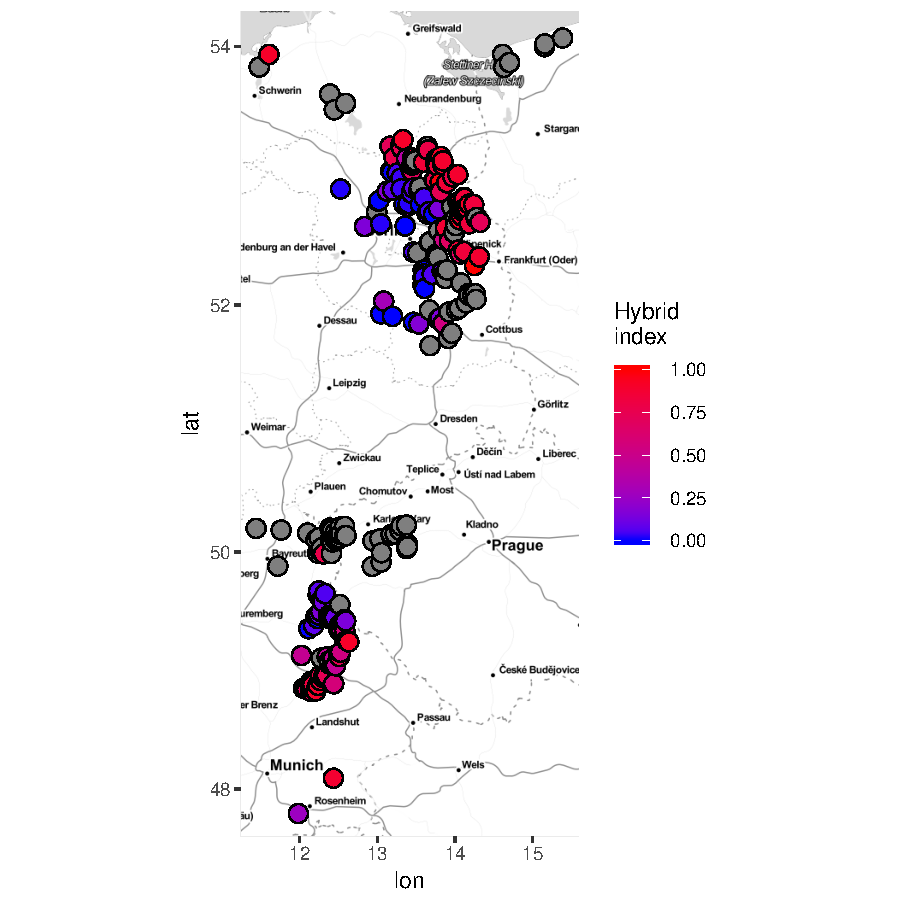
\includegraphics[width=.6\linewidth]{figure/Data-Analysis-Alice-2017-Rnwauto-report-1} 

}


\begin{kframe}\begin{alltt}
\hlcom{# ***************************************************************}

\hlcom{# If the same cluster was sampled several time one year, we sum the mice caught}
\hlstd{aggdata} \hlkwb{<-} \hlkwd{aggregate}\hlstd{(}\hlkwc{x} \hlstd{= TrapTable[}\hlkwd{c}\hlstd{(}\hlstr{"Number_mus_caught"}\hlstd{,} \hlstr{"Number_traps_set"}\hlstd{)],}
                     \hlkwc{by} \hlstd{= TrapTable[}\hlkwd{c}\hlstd{(}\hlstr{"Latitude"}\hlstd{,} \hlstr{"Longitude"}\hlstd{,} \hlstr{"Year"}\hlstd{)],} \hlkwc{FUN} \hlstd{= sum)}

\hlkwd{names}\hlstd{(aggdata)[}\hlkwd{names}\hlstd{(aggdata)} \hlopt{==} \hlstr{"x"}\hlstd{]} \hlkwb{<-} \hlstr{"Number_mice_caught"}

\hlcom{# add a counter for the localities:}
\hlstd{aggdata} \hlkwb{<-} \hlkwd{as.data.table}\hlstd{(aggdata)[, count} \hlkwb{:=} \hlkwd{seq}\hlstd{(.N),} \hlkwc{by} \hlstd{=} \hlkwd{c}\hlstd{(}\hlstr{"Latitude"}\hlstd{,} \hlstr{"Longitude"}\hlstd{)][]}

\hlcom{# density of mice in 100%}
\hlstd{aggdata}\hlopt{$}\hlstd{density} \hlkwb{<-} \hlstd{aggdata}\hlopt{$}\hlstd{Number_mus_caught} \hlopt{/} \hlstd{aggdata}\hlopt{$}\hlstd{Number_traps_set} \hlopt{*}\hlnum{100}

\hlcom{# so you define new and old localities:}
\hlstd{aggdata}\hlopt{$}\hlstd{is.new.loc} \hlkwb{<-} \hlstr{"new"}
\hlstd{aggdata[aggdata}\hlopt{$}\hlstd{count} \hlopt{!=} \hlnum{1}\hlstd{,} \hlstr{"is.new.loc"}\hlstd{]} \hlkwb{<-} \hlstr{"old"}

\hlcom{# NB : in 2016 and 2017 we have the trapping attemps, not the other years}
\hlcom{# ***************************************************************}

\hlcom{# density of mice added to MiceTable}
\hlstd{TotalTable} \hlkwb{<-} \hlkwd{merge}\hlstd{(MiceTable, aggdata,} \hlkwc{all} \hlstd{=} \hlnum{TRUE}\hlstd{)}

\hlstd{TotalTable} \hlkwb{<-} \hlstd{TotalTable[TotalTable}\hlopt{$}\hlstd{Longitude} \hlopt{<} \hlnum{17}\hlstd{,]}
\hlcom{# ***************************************************************}

\hlcom{# body mass index as log body mass/log body length (Hayes et al. 2014)}
\hlstd{TotalTable}\hlopt{$}\hlstd{BMI} \hlkwb{<-} \hlkwd{log}\hlstd{(TotalTable}\hlopt{$}\hlstd{Body_weight)} \hlopt{/} \hlkwd{log}\hlstd{(TotalTable}\hlopt{$}\hlstd{Body_length)}

\hlcom{# ***************************************************************}

\hlcom{# how many localities (new and old) sampled per year? }

\hlcom{# barplot }
\hlkwd{ggplot}\hlstd{(}\hlkwc{data}\hlstd{=}\hlkwd{data.frame}\hlstd{(}\hlkwd{table}\hlstd{(aggdata}\hlopt{$}\hlstd{Year, aggdata}\hlopt{$}\hlstd{is.new.loc)),}
       \hlkwd{aes}\hlstd{(}\hlkwc{x}\hlstd{=Var1,} \hlkwc{y}\hlstd{=Freq,} \hlkwc{fill}\hlstd{=Var2))} \hlopt{+}
  \hlkwd{geom_bar}\hlstd{(}\hlkwc{stat}\hlstd{=}\hlstr{"identity"}\hlstd{)}\hlopt{+}
  \hlkwd{geom_text}\hlstd{(}\hlkwd{aes}\hlstd{(}\hlkwc{y}\hlstd{=Freq,} \hlkwc{label}\hlstd{=Freq),} \hlkwc{vjust}\hlstd{=}\hlnum{1.6}\hlstd{,}
            \hlkwc{color}\hlstd{=}\hlstr{"white"}\hlstd{,} \hlkwc{size}\hlstd{=}\hlnum{6}\hlstd{)}\hlopt{+}
  \hlkwd{scale_fill_brewer}\hlstd{(}\hlkwc{palette}\hlstd{=}\hlstr{"Paired"}\hlstd{)}\hlopt{+}
  \hlkwd{theme_classic}\hlstd{()}
\end{alltt}
\end{kframe}

{\centering 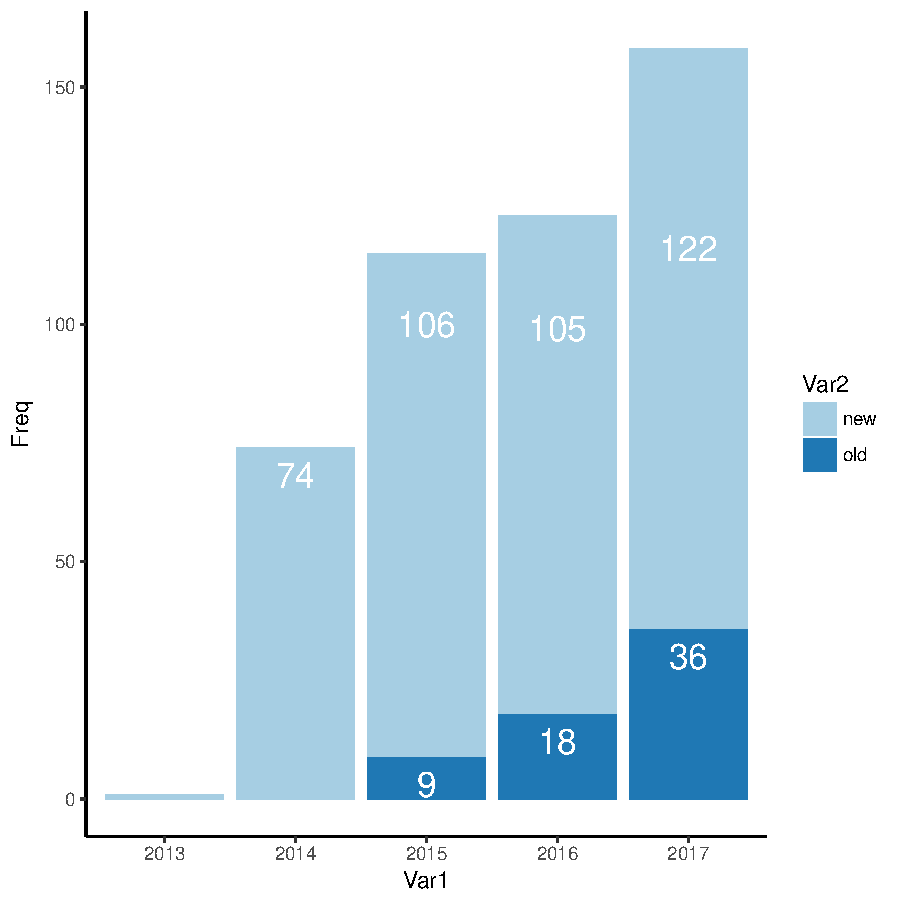
\includegraphics[width=.6\linewidth]{figure/Data-Analysis-Alice-2017-Rnwauto-report-2} 

}


\begin{kframe}\begin{alltt}
\hlcom{# how many mice where caught every year?}
\hlstd{aggmice} \hlkwb{<-} \hlkwd{aggregate}\hlstd{(}\hlkwc{x} \hlstd{= TrapTable[}\hlkwd{c}\hlstd{(}\hlstr{"Number_mus_caught"}\hlstd{)],}
                     \hlkwc{by} \hlstd{= TrapTable[}\hlkwd{c}\hlstd{(}\hlstr{"Year"}\hlstd{)],} \hlkwc{FUN} \hlstd{= sum)}

\hlkwd{ggplot}\hlstd{(aggmice,} \hlkwd{aes}\hlstd{(}\hlkwc{x} \hlstd{=} \hlkwd{factor}\hlstd{(Year),} \hlkwc{y} \hlstd{= Number_mus_caught))}\hlopt{+}
  \hlkwd{geom_bar}\hlstd{(}\hlkwc{stat}\hlstd{=}\hlstr{"identity"}\hlstd{,} \hlkwc{width}\hlstd{=}\hlnum{0.7}\hlstd{,} \hlkwc{color}\hlstd{=}\hlstr{"black"}\hlstd{,} \hlkwc{fill} \hlstd{=} \hlstr{"orange"}\hlstd{)}\hlopt{+}
  \hlkwd{theme_classic}\hlstd{(}\hlkwc{base_size} \hlstd{=} \hlnum{18}\hlstd{)} \hlopt{+}
  \hlkwd{theme}\hlstd{(}\hlkwc{axis.title.y}\hlstd{=}\hlkwd{element_blank}\hlstd{(),} \hlkwc{axis.title.x}\hlstd{=}\hlkwd{element_blank}\hlstd{())} \hlopt{+}
  \hlkwd{ggtitle}\hlstd{(}\hlkwc{label} \hlstd{=} \hlstr{"Number of mice caught per year"}\hlstd{)} \hlopt{+}
  \hlkwd{geom_text}\hlstd{(}\hlkwd{aes}\hlstd{(}\hlkwc{label}\hlstd{=Number_mus_caught),} \hlkwc{vjust}\hlstd{=}\hlnum{1.6}\hlstd{,} \hlkwc{color}\hlstd{=}\hlstr{"black"}\hlstd{,} \hlkwc{size}\hlstd{=}\hlnum{10}\hlstd{)}\hlopt{+}
  \hlkwd{theme}\hlstd{(}\hlkwc{legend.title}\hlstd{=}\hlkwd{element_blank}\hlstd{())}
\end{alltt}
\end{kframe}

{\centering 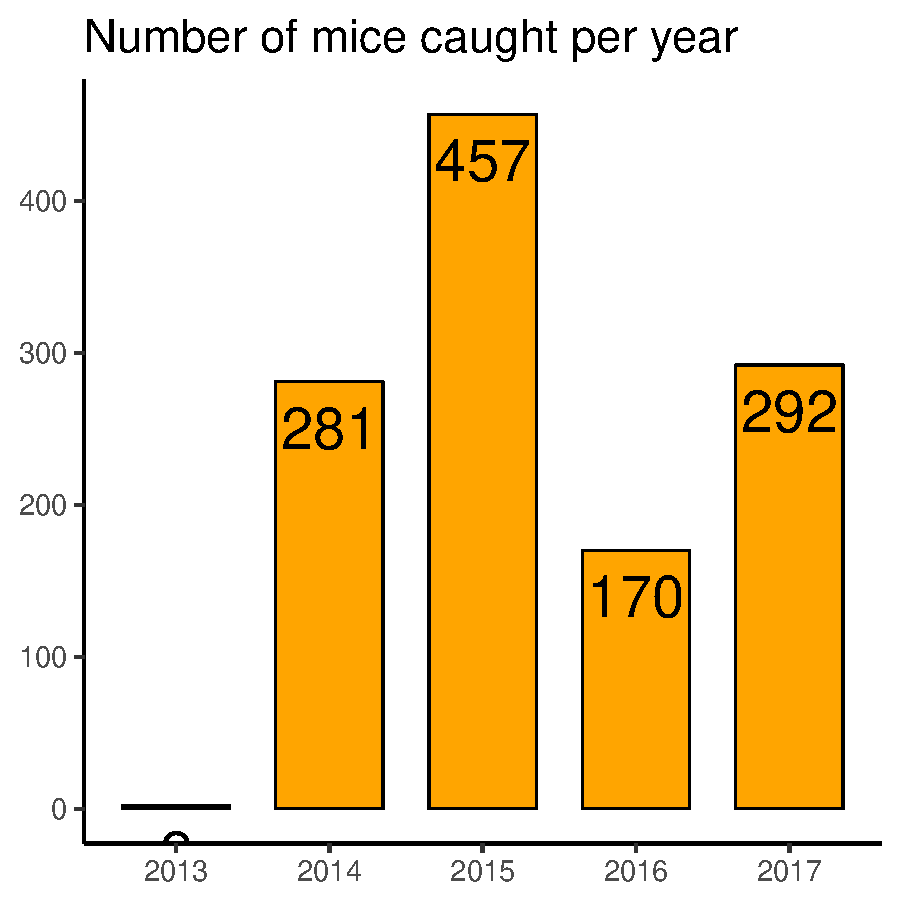
\includegraphics[width=.6\linewidth]{figure/Data-Analysis-Alice-2017-Rnwauto-report-3} 

}


\begin{kframe}\begin{alltt}
\hlcom{# Number of localities with 1, 2, 3 or more mice caught over the years}
\hlkwd{ggplot}\hlstd{(aggdata,} \hlkwd{aes}\hlstd{(}\hlkwc{x} \hlstd{= Number_mus_caught))} \hlopt{+}
  \hlkwd{geom_histogram}\hlstd{(}\hlkwc{fill}\hlstd{=}\hlstr{"black"}\hlstd{,} \hlkwc{col}\hlstd{=}\hlstr{"grey"}\hlstd{,} \hlkwc{binwidth} \hlstd{=} \hlnum{1}\hlstd{)} \hlopt{+}
  \hlkwd{ggtitle}\hlstd{(}\hlkwc{label} \hlstd{=} \hlstr{"Histogram of # mice caught per locality"}\hlstd{)}\hlopt{+}
  \hlkwd{theme_classic}\hlstd{(}\hlkwc{base_size} \hlstd{=} \hlnum{18}\hlstd{)} \hlopt{+}
  \hlkwd{labs}\hlstd{(}\hlkwc{x} \hlstd{=} \hlstr{"Number of mice caught"}\hlstd{)}
\end{alltt}
\end{kframe}

{\centering 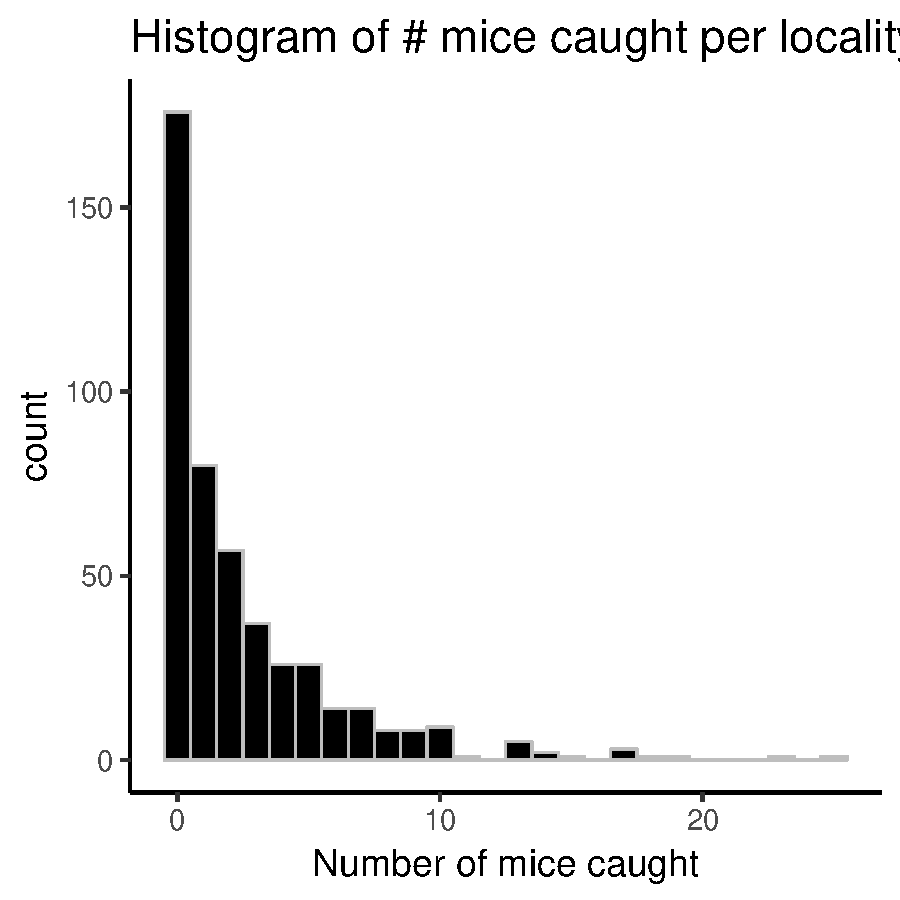
\includegraphics[width=.6\linewidth]{figure/Data-Analysis-Alice-2017-Rnwauto-report-4} 

}


\begin{kframe}\begin{alltt}
\hlcom{# ***************************************************************}
\hlcom{# test potential linear correlation}
\hlkwd{library}\hlstd{(devtools)}
\hlkwd{install_github}\hlstd{(}\hlstr{"hadley/ggplot2"}\hlstd{)}
\end{alltt}


{\ttfamily\noindent\itshape\color{messagecolor}{\#\# Skipping install of 'ggplot2' from a github remote, the SHA1 (582acfec) has not changed since last install.\\\#\#\ \  Use `force = TRUE` to force installation}}\begin{alltt}
\hlkwd{install_github}\hlstd{(}\hlstr{"ggobi/ggally"}\hlstd{)}
\end{alltt}


{\ttfamily\noindent\itshape\color{messagecolor}{\#\# Skipping install of 'GGally' from a github remote, the SHA1 (0dc3283a) has not changed since last install.\\\#\#\ \  Use `force = TRUE` to force installation}}\begin{alltt}
\hlkwd{library}\hlstd{(GGally)}

\hlkwd{ggpairs}\hlstd{(}
  \hlstd{TotalTable,} \hlkwd{which}\hlstd{(}\hlkwd{names}\hlstd{(TotalTable)} \hlopt \hlkwd{c}\hlstd{(}\hlstr{"Year"}\hlstd{,}\hlstr{"HI"}\hlstd{,} \hlstr{"density"}\hlstd{,} \hlstr{"BMI"}\hlstd{)),}
  \hlkwc{upper} \hlstd{=} \hlkwd{list}\hlstd{(}
    \hlkwc{continuous} \hlstd{=} \hlkwd{wrap}\hlstd{(}\hlstr{'cor'}\hlstd{,} \hlkwc{method} \hlstd{=} \hlstr{"spearman"}\hlstd{)}
  \hlstd{),}
  \hlkwc{lower} \hlstd{=} \hlkwd{list}\hlstd{(}
    \hlkwc{continuous} \hlstd{=} \hlstr{'cor'}
  \hlstd{)}
\hlstd{)}
\end{alltt}


{\ttfamily\noindent\color{warningcolor}{\#\# Warning in (function (data, mapping, alignPercent = 0.6, method = "{}pearson"{}, : Removed 689 rows containing missing values}}

{\ttfamily\noindent\color{warningcolor}{\#\# Warning in (function (data, mapping, alignPercent = 0.6, method = "{}pearson"{}, : Removed 762 rows containing missing values}}

{\ttfamily\noindent\color{warningcolor}{\#\# Warning in (function (data, mapping, alignPercent = 0.6, method = "{}pearson"{}, : Removed 548 rows containing missing values}}

{\ttfamily\noindent\color{warningcolor}{\#\# Warning in (function (data, mapping, alignPercent = 0.6, method = "{}pearson"{}, : Removed 689 rows containing missing values}}

{\ttfamily\noindent\color{warningcolor}{\#\# Warning: Removed 689 rows containing non-finite values (stat\_density).}}

{\ttfamily\noindent\color{warningcolor}{\#\# Warning in (function (data, mapping, alignPercent = 0.6, method = "{}pearson"{}, : Removed 1231 rows containing missing values}}

{\ttfamily\noindent\color{warningcolor}{\#\# Warning in (function (data, mapping, alignPercent = 0.6, method = "{}pearson"{}, : Removed 761 rows containing missing values}}

{\ttfamily\noindent\color{warningcolor}{\#\# Warning in (function (data, mapping, alignPercent = 0.6, method = "{}pearson"{}, : Removed 762 rows containing missing values}}

{\ttfamily\noindent\color{warningcolor}{\#\# Warning in (function (data, mapping, alignPercent = 0.6, method = "{}pearson"{}, : Removed 1231 rows containing missing values}}

{\ttfamily\noindent\color{warningcolor}{\#\# Warning: Removed 762 rows containing non-finite values (stat\_density).}}

{\ttfamily\noindent\color{warningcolor}{\#\# Warning in (function (data, mapping, alignPercent = 0.6, method = "{}pearson"{}, : Removed 1216 rows containing missing values}}

{\ttfamily\noindent\color{warningcolor}{\#\# Warning in (function (data, mapping, alignPercent = 0.6, method = "{}pearson"{}, : Removed 548 rows containing missing values}}

{\ttfamily\noindent\color{warningcolor}{\#\# Warning in (function (data, mapping, alignPercent = 0.6, method = "{}pearson"{}, : Removed 761 rows containing missing values}}

{\ttfamily\noindent\color{warningcolor}{\#\# Warning in (function (data, mapping, alignPercent = 0.6, method = "{}pearson"{}, : Removed 1216 rows containing missing values}}

{\ttfamily\noindent\color{warningcolor}{\#\# Warning: Removed 548 rows containing non-finite values (stat\_density).}}\end{kframe}

{\centering 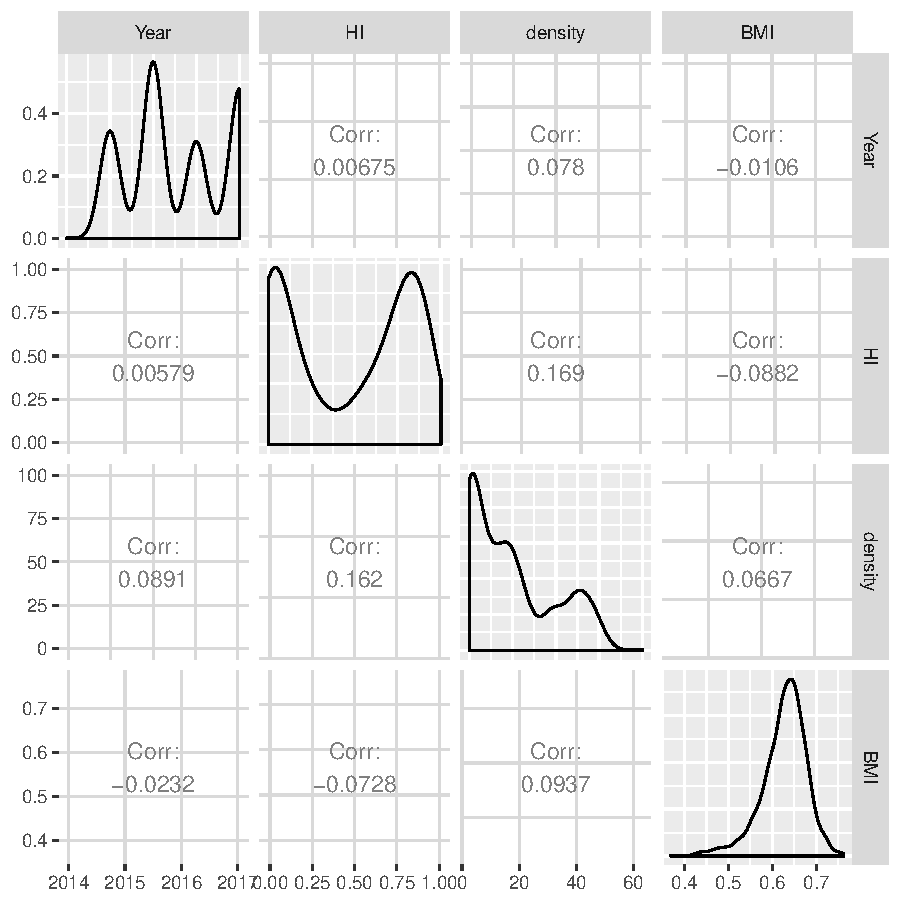
\includegraphics[width=.6\linewidth]{figure/Data-Analysis-Alice-2017-Rnwauto-report-5} 

}


\begin{kframe}\begin{alltt}
\hlkwd{ggcorr}\hlstd{(TotalTable[(}\hlkwd{names}\hlstd{(TotalTable)} \hlopt \hlkwd{c}\hlstd{(}\hlstr{"Year"}\hlstd{,} \hlstr{"HI"}\hlstd{,} \hlstr{"density"}\hlstd{,} \hlstr{"BMI"}\hlstd{))],}
       \hlkwc{palette} \hlstd{=} \hlstr{"RdBu"}\hlstd{,} \hlkwc{label} \hlstd{=} \hlnum{TRUE}\hlstd{,} \hlkwc{method} \hlstd{=} \hlkwd{c}\hlstd{(}\hlstr{"pairwise"}\hlstd{,} \hlstr{"spearman"}\hlstd{))} \hlopt{+}
  \hlkwd{ggtitle}\hlstd{(}\hlstr{"Pairwise correlations with Spearman coefficient"}\hlstd{)}
\end{alltt}
\end{kframe}

{\centering 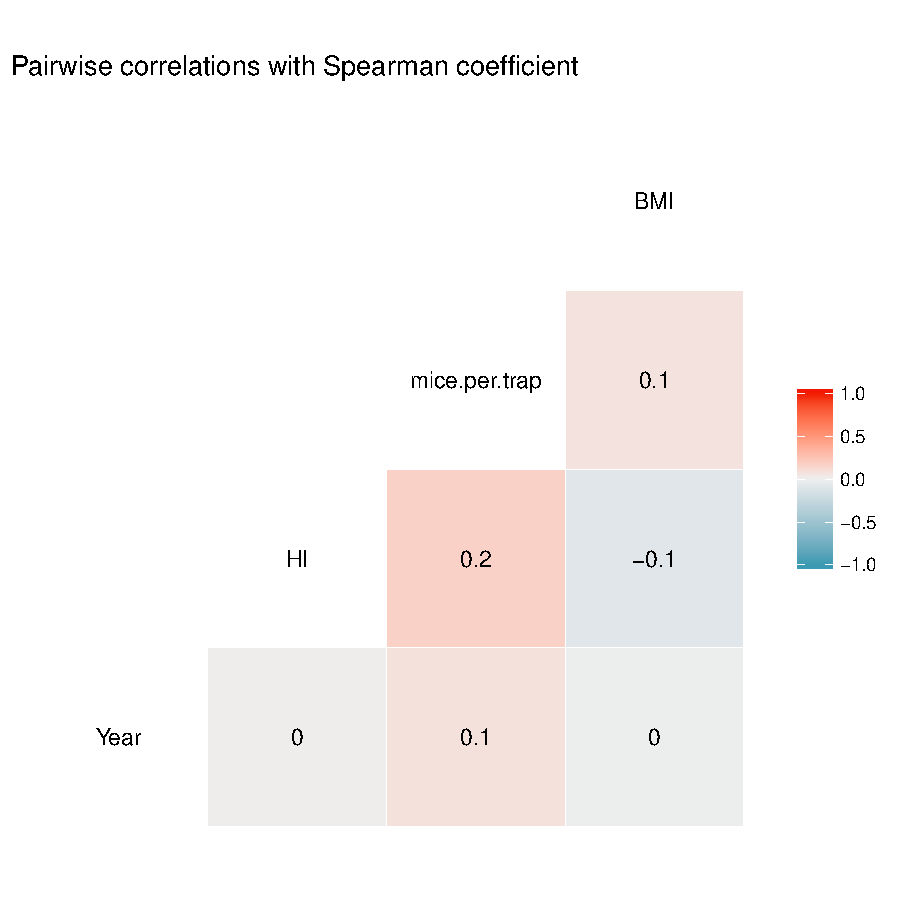
\includegraphics[width=.6\linewidth]{figure/Data-Analysis-Alice-2017-Rnwauto-report-6} 

}


\begin{kframe}\begin{alltt}
\hlcom{# Sex - localities }
\hlkwd{ggplot}\hlstd{(TotalTable[TotalTable}\hlopt{$}\hlstd{Sex} \hlopt \hlkwd{c}\hlstd{(}\hlstr{"M"}\hlstd{,} \hlstr{"F"}\hlstd{), ],} \hlkwd{aes}\hlstd{(}\hlkwc{x} \hlstd{= Longitude,} \hlkwc{y} \hlstd{= Latitude,} \hlkwc{fill} \hlstd{= Sex))} \hlopt{+}
  \hlkwd{theme_classic}\hlstd{(}\hlkwc{base_size} \hlstd{=} \hlnum{18}\hlstd{)} \hlopt{+}
  \hlkwd{theme}\hlstd{(}\hlkwc{axis.title.y}\hlstd{=}\hlkwd{element_blank}\hlstd{(),} \hlkwc{axis.title.x}\hlstd{=}\hlkwd{element_blank}\hlstd{())} \hlopt{+}
  \hlkwd{ggtitle}\hlstd{(}\hlkwc{label} \hlstd{=} \hlstr{"Cluster of males and female per localities"}\hlstd{)} \hlopt{+}
  \hlkwd{theme}\hlstd{(}\hlkwc{legend.title}\hlstd{=}\hlkwd{element_blank}\hlstd{())} \hlopt{+}
  \hlkwd{scale_fill_manual}\hlstd{(}\hlkwc{values} \hlstd{=} \hlkwd{c}\hlstd{(}\hlstr{"pink"}\hlstd{,} \hlstr{"blue"}\hlstd{))} \hlopt{+}
  \hlkwd{geom_density2d}\hlstd{(}\hlkwd{aes}\hlstd{(}\hlkwc{color} \hlstd{= Sex),} \hlkwc{size} \hlstd{=} \hlnum{1}\hlstd{)} \hlopt{+}
  \hlkwd{geom_point}\hlstd{(}\hlkwc{col} \hlstd{=} \hlstr{"black"}\hlstd{,} \hlkwc{size} \hlstd{=} \hlnum{4}\hlstd{,} \hlkwc{pch} \hlstd{=} \hlnum{21}\hlstd{)}
\end{alltt}
\end{kframe}

{\centering 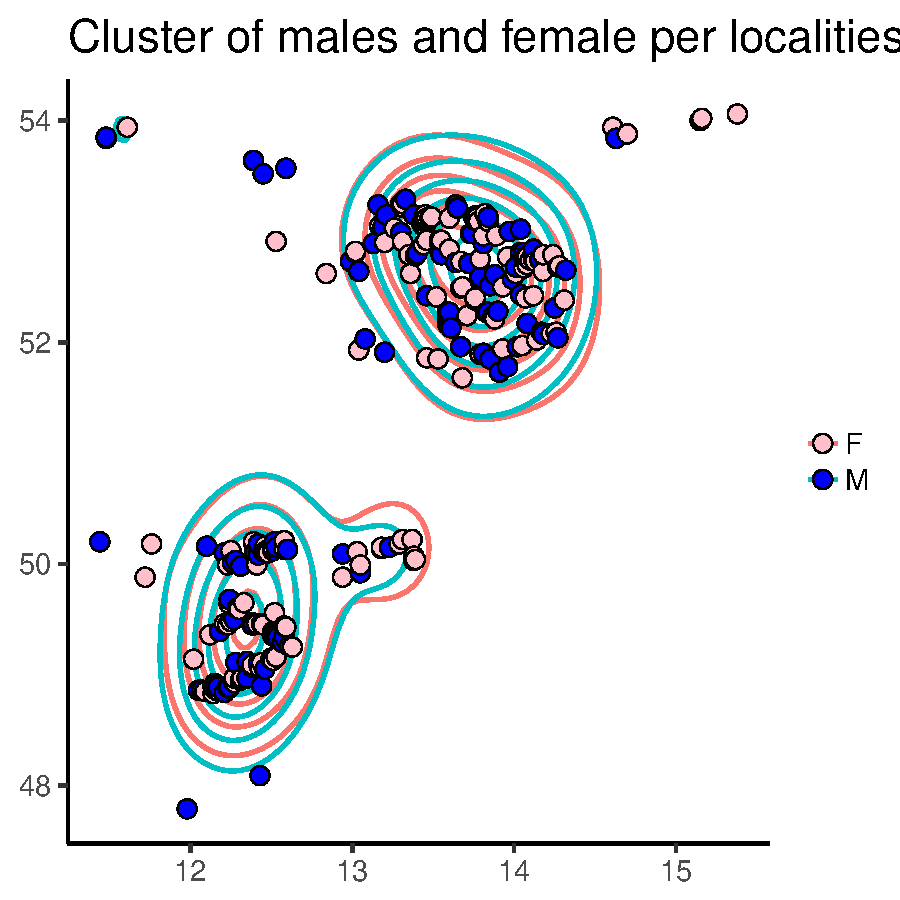
\includegraphics[width=.6\linewidth]{figure/Data-Analysis-Alice-2017-Rnwauto-report-7} 

}


\begin{kframe}\begin{alltt}
\hlcom{# Host density - sex}
\hlkwd{ggplot}\hlstd{(TotalTable[TotalTable}\hlopt{$}\hlstd{Sex} \hlopt \hlkwd{c}\hlstd{(}\hlstr{"M"}\hlstd{,} \hlstr{"F"}\hlstd{),],} \hlkwd{aes}\hlstd{(}\hlkwc{x} \hlstd{= density))}\hlopt{+}
  \hlkwd{geom_bar}\hlstd{(}\hlkwd{aes}\hlstd{(}\hlkwc{fill} \hlstd{= Sex),} \hlkwc{stat} \hlstd{=} \hlstr{"count"}\hlstd{,} \hlkwc{binwidth} \hlstd{=} \hlnum{3}\hlstd{,} \hlkwc{col} \hlstd{=} \hlstr{"white"}\hlstd{)} \hlopt{+}
  \hlkwd{theme_classic}\hlstd{()}
\end{alltt}


{\ttfamily\noindent\color{warningcolor}{\#\# Warning: `geom\_bar()` no longer has a `binwidth` parameter. Please use `geom\_histogram()` instead.}}

{\ttfamily\noindent\color{warningcolor}{\#\# Warning: Removed 761 rows containing non-finite values (stat\_bin).}}\end{kframe}

{\centering 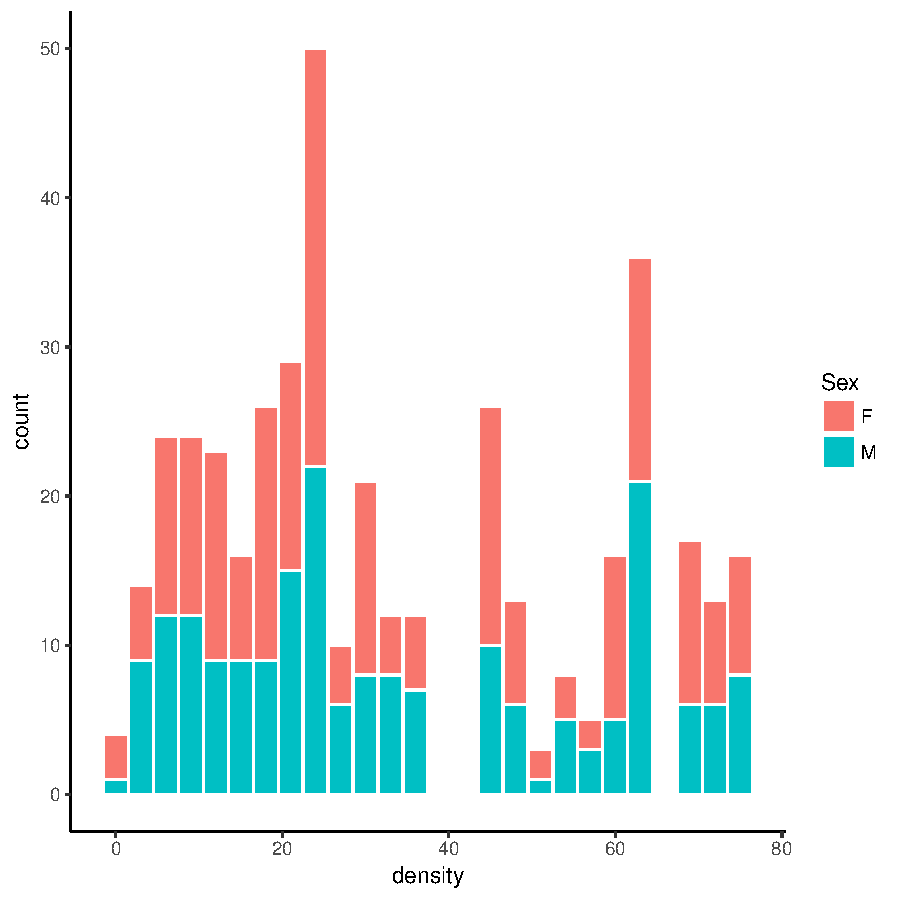
\includegraphics[width=.6\linewidth]{figure/Data-Analysis-Alice-2017-Rnwauto-report-8} 

}


\begin{kframe}\begin{alltt}
\hlcom{# BMI - subspecies}
\hlstd{TotalTable}\hlopt{$}\hlstd{subspecies[TotalTable}\hlopt{$}\hlstd{HI} \hlopt{<} \hlnum{0.1}\hlstd{]} \hlkwb{<-} \hlstr{"Mmd"}
\hlstd{TotalTable}\hlopt{$}\hlstd{subspecies[TotalTable}\hlopt{$}\hlstd{HI} \hlopt{>=} \hlnum{0.9}\hlstd{]} \hlkwb{<-} \hlstr{"Mmm"}

\hlcom{# Density plots }
\hlkwd{ggplot}\hlstd{(TotalTable[}\hlopt{!}\hlkwd{is.na}\hlstd{(TotalTable}\hlopt{$}\hlstd{subspecies),],} \hlkwd{aes}\hlstd{(}\hlkwc{x} \hlstd{= BMI,} \hlkwc{fill} \hlstd{= subspecies))} \hlopt{+}
  \hlkwd{geom_density}\hlstd{(}\hlkwc{alpha}\hlstd{=}\hlnum{.3}\hlstd{)} \hlopt{+}
  \hlkwd{scale_fill_manual}\hlstd{(}\hlkwc{values} \hlstd{=} \hlkwd{c}\hlstd{(}\hlstr{"blue"}\hlstd{,} \hlstr{"red"}\hlstd{))}
\end{alltt}


{\ttfamily\noindent\color{warningcolor}{\#\# Warning: Removed 38 rows containing non-finite values (stat\_density).}}\end{kframe}

{\centering 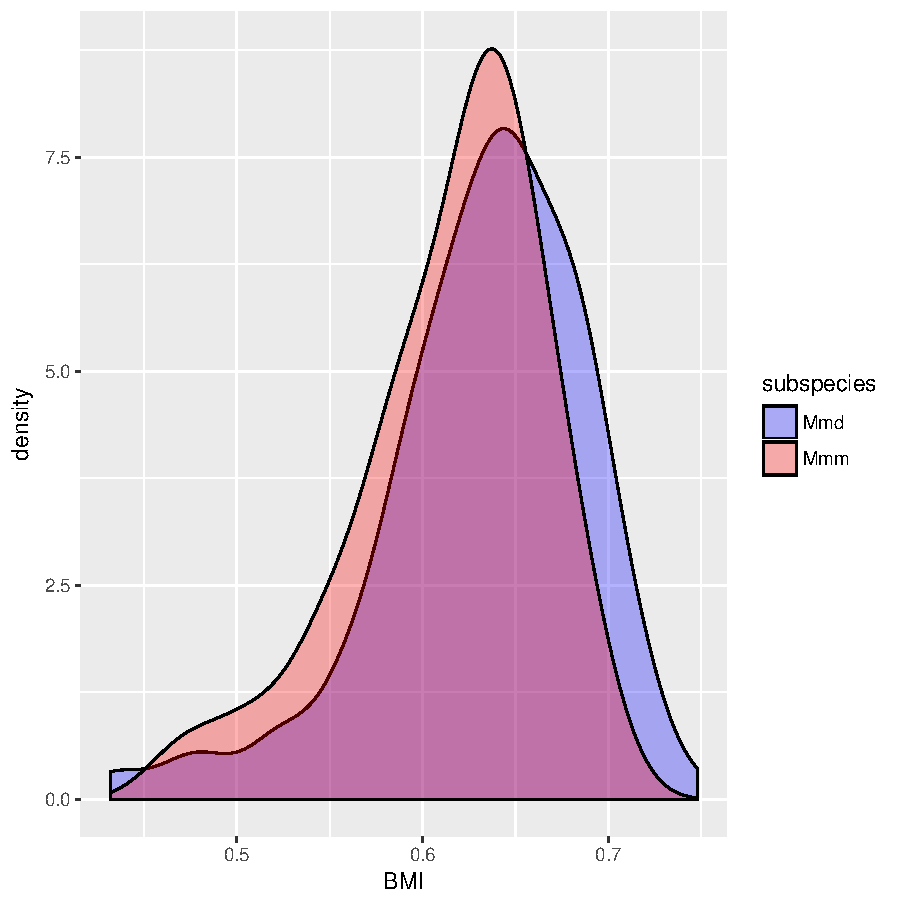
\includegraphics[width=.6\linewidth]{figure/Data-Analysis-Alice-2017-Rnwauto-report-9} 

}


\begin{kframe}\begin{alltt}
\hlkwd{ggplot}\hlstd{(TotalTable[}\hlopt{!}\hlkwd{is.na}\hlstd{(TotalTable}\hlopt{$}\hlstd{subspecies),],} \hlkwd{aes}\hlstd{(}\hlkwc{x}\hlstd{=subspecies,} \hlkwc{y} \hlstd{= BMI,} \hlkwc{fill}\hlstd{=subspecies))} \hlopt{+}
  \hlkwd{geom_boxplot}\hlstd{()} \hlopt{+}
  \hlkwd{guides}\hlstd{(}\hlkwc{fill}\hlstd{=}\hlnum{FALSE}\hlstd{)} \hlopt{+}
  \hlkwd{scale_fill_manual}\hlstd{(}\hlkwc{values} \hlstd{=} \hlkwd{c}\hlstd{(}\hlstr{"blue"}\hlstd{,} \hlstr{"red"}\hlstd{))} \hlopt{+}
  \hlkwd{theme_classic}\hlstd{()}
\end{alltt}


{\ttfamily\noindent\color{warningcolor}{\#\# Warning: Removed 38 rows containing non-finite values (stat\_boxplot).}}\end{kframe}

{\centering 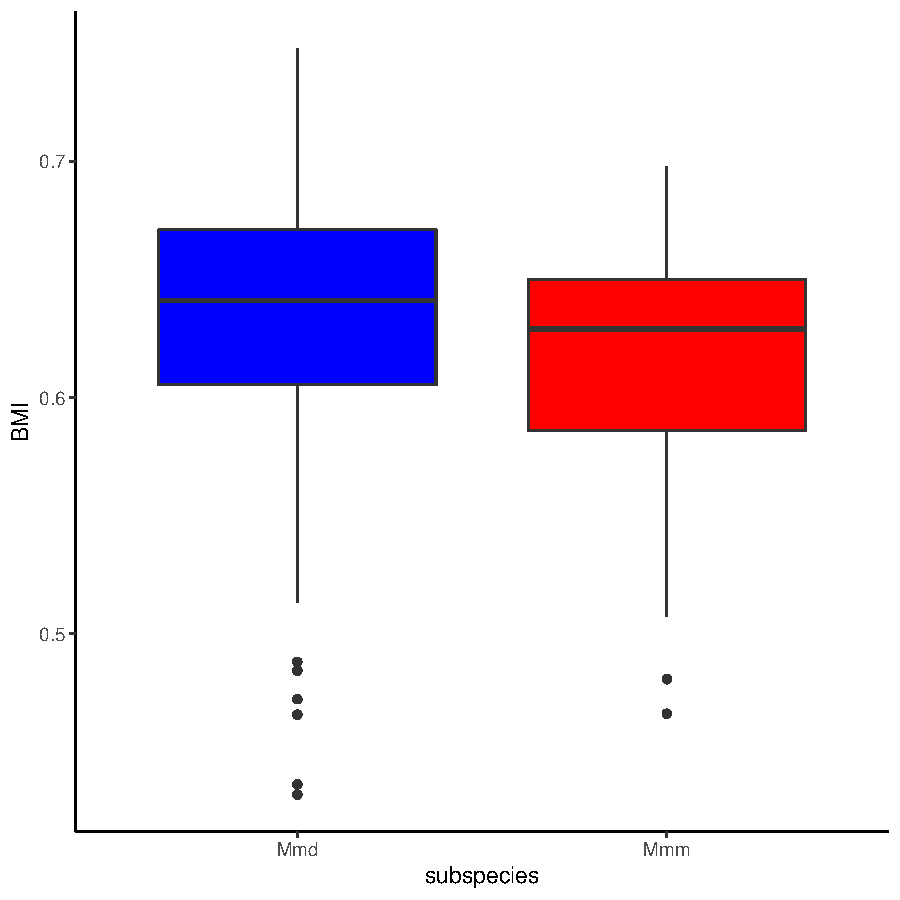
\includegraphics[width=.6\linewidth]{figure/Data-Analysis-Alice-2017-Rnwauto-report-10} 

}


\begin{kframe}\begin{alltt}
\hlcom{# Host density - hybrid index}
\hlkwd{ggplot}\hlstd{(TotalTable[}\hlopt{!}\hlkwd{is.na}\hlstd{(TotalTable}\hlopt{$}\hlstd{HI),],} \hlkwd{aes}\hlstd{(}\hlkwc{x} \hlstd{= HI,} \hlkwc{y} \hlstd{= density))}\hlopt{+}
  \hlkwd{geom_point}\hlstd{(}\hlkwc{pch} \hlstd{=} \hlnum{21}\hlstd{)}\hlopt{+}
  \hlkwd{geom_smooth}\hlstd{(}\hlkwc{col} \hlstd{=} \hlstr{"red"}\hlstd{)} \hlopt{+}
  \hlkwd{theme_classic}\hlstd{()}
\end{alltt}


{\ttfamily\noindent\itshape\color{messagecolor}{\#\# `geom\_smooth()` using method = 'loess' and formula 'y \textasciitilde{} x'}}

{\ttfamily\noindent\color{warningcolor}{\#\# Warning: Removed 542 rows containing non-finite values (stat\_smooth).}}

{\ttfamily\noindent\color{warningcolor}{\#\# Warning: Removed 542 rows containing missing values (geom\_point).}}\end{kframe}

{\centering 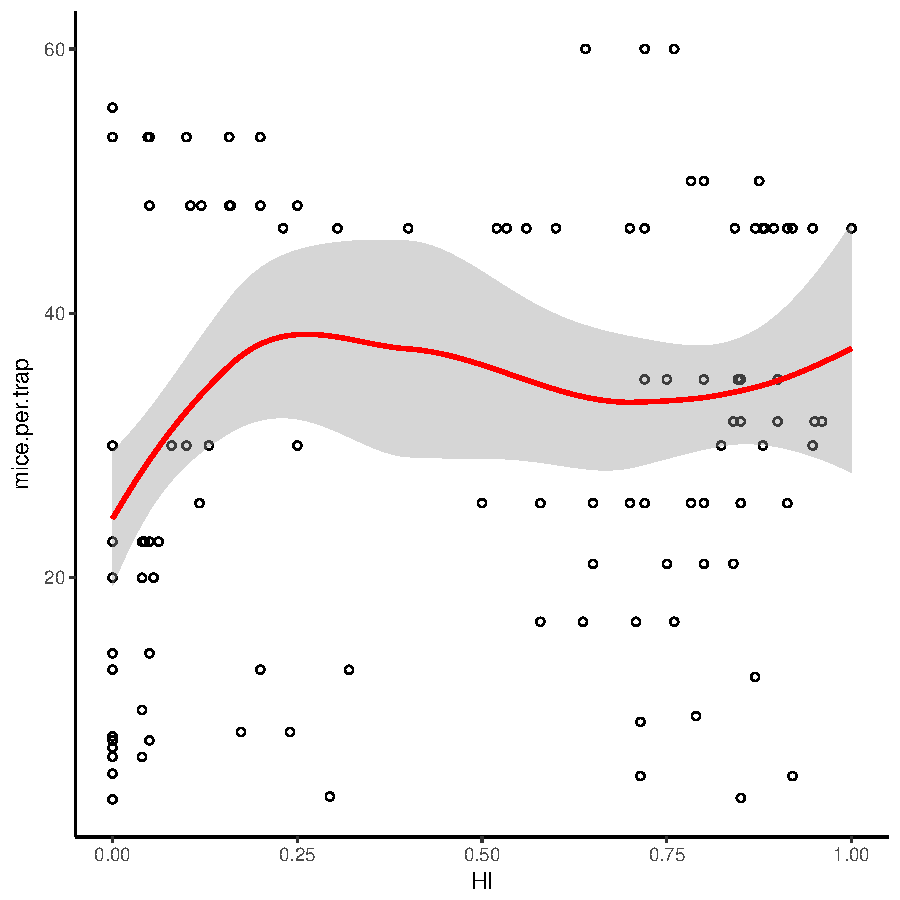
\includegraphics[width=.6\linewidth]{figure/Data-Analysis-Alice-2017-Rnwauto-report-11} 

}


\begin{kframe}\begin{alltt}
\hlkwd{ggplot}\hlstd{(TotalTable[}\hlopt{!}\hlkwd{is.na}\hlstd{(TotalTable}\hlopt{$}\hlstd{HI),],} \hlkwd{aes}\hlstd{(}\hlkwc{x} \hlstd{= HI,} \hlkwc{y} \hlstd{= density))}\hlopt{+}
  \hlkwd{geom_point}\hlstd{(}\hlkwc{pch} \hlstd{=} \hlnum{21}\hlstd{)}\hlopt{+}
  \hlkwd{geom_smooth}\hlstd{(}\hlkwc{col} \hlstd{=} \hlstr{"red"}\hlstd{,} \hlkwc{method} \hlstd{=} \hlstr{"lm"}\hlstd{)} \hlopt{+}
  \hlkwd{theme_classic}\hlstd{()}
\end{alltt}


{\ttfamily\noindent\color{warningcolor}{\#\# Warning: Removed 542 rows containing non-finite values (stat\_smooth).}}

{\ttfamily\noindent\color{warningcolor}{\#\# Warning: Removed 542 rows containing missing values (geom\_point).}}\end{kframe}

{\centering 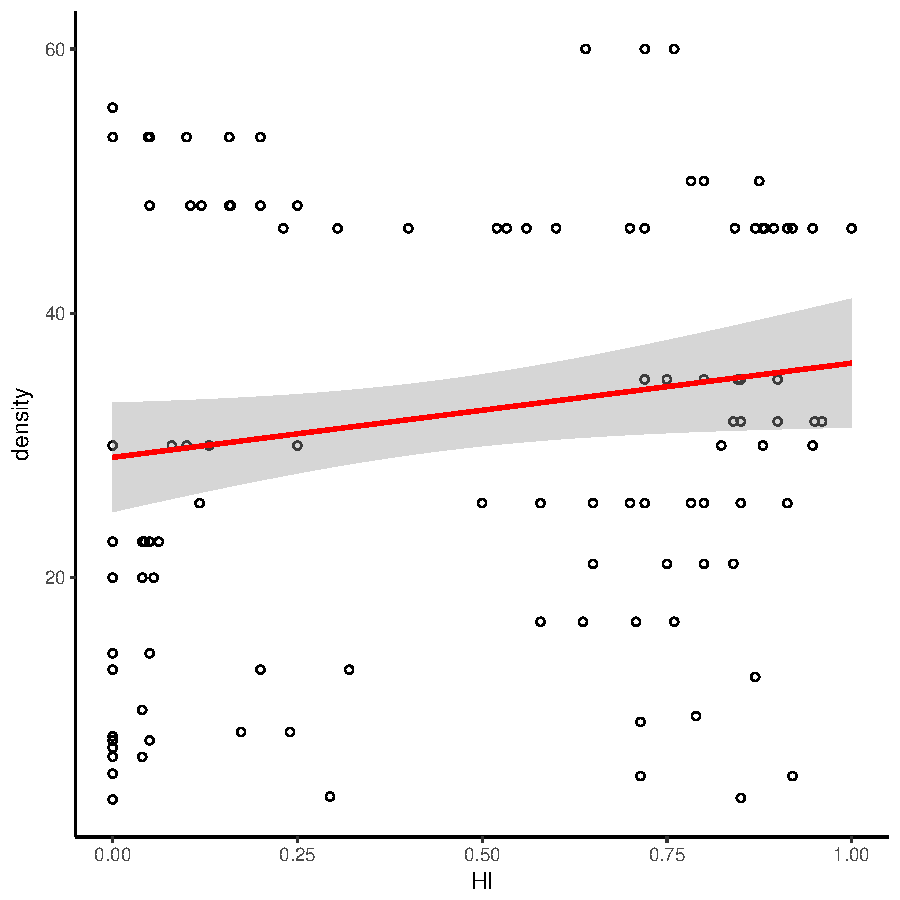
\includegraphics[width=.6\linewidth]{figure/Data-Analysis-Alice-2017-Rnwauto-report-12} 

}


\begin{kframe}\begin{alltt}
\hlcom{# ***************************************************************}
\hlcom{# Parasites}
\hlstd{WormsDF} \hlkwb{<-} \hlstd{TotalTable[}\hlkwd{c}\hlstd{(}\hlstr{"Mouse_ID"}\hlstd{,} \hlstr{"Cysticercus"}\hlstd{,} \hlstr{"Trichuris_muris"}\hlstd{,} \hlstr{"Aspiculuris_tetraptera"}\hlstd{,} \hlstr{"Syphacia_obvelata"}\hlstd{,}
                        \hlstr{"Mastophorus_muris"}\hlstd{,} \hlstr{"Heterakis_spumosa"}\hlstd{,} \hlstr{"Mesocestoides"}\hlstd{,}
                        \hlstr{"Catenotaenia_pusilla"}\hlstd{,} \hlstr{"Hymenolepis"}\hlstd{,} \hlstr{"Oxyurids"}\hlstd{,} \hlstr{"Mix_Syphacia_Aspiculuris"}\hlstd{,}
                        \hlstr{"Heligmosomoides_polygurus"}\hlstd{,} \hlstr{"Latitude"}\hlstd{,} \hlstr{"Longitude"}\hlstd{)]}

\hlcom{# ("Hymenolepis_microstoma", "Hymenolepis_diminiuta") to check, contains "TRUE" and "FALSE"}

\hlstd{WormsDF} \hlkwb{<-} \hlkwd{na.omit}\hlstd{(}\hlkwd{melt}\hlstd{(WormsDF,} \hlkwc{id} \hlstd{=} \hlkwd{c}\hlstd{(}\hlstr{"Mouse_ID"}\hlstd{,} \hlstr{"Longitude"}\hlstd{,} \hlstr{"Latitude"}\hlstd{)))}

\hlstd{aggworms} \hlkwb{<-} \hlkwd{aggregate}\hlstd{(}\hlkwc{x} \hlstd{= WormsDF[}\hlstr{"value"}\hlstd{],}
                      \hlkwc{by} \hlstd{= WormsDF[}\hlstr{"variable"}\hlstd{],} \hlkwc{FUN} \hlstd{= length)}

\hlkwd{ggplot}\hlstd{(}\hlkwc{data}\hlstd{=aggworms,} \hlkwd{aes}\hlstd{(}\hlkwc{x}\hlstd{=variable,} \hlkwc{y}\hlstd{=value))} \hlopt{+}
  \hlkwd{geom_bar}\hlstd{(}\hlkwc{stat}\hlstd{=}\hlstr{"identity"}\hlstd{,} \hlkwc{fill} \hlstd{=} \hlstr{"#B983FF"}\hlstd{,} \hlkwc{col} \hlstd{=} \hlstr{"grey"}\hlstd{)} \hlopt{+}
  \hlkwd{theme_classic}\hlstd{()} \hlopt{+}
  \hlkwd{theme}\hlstd{(}\hlkwc{axis.text.x} \hlstd{=} \hlkwd{element_text}\hlstd{(}\hlkwc{angle} \hlstd{=} \hlnum{45}\hlstd{,} \hlkwc{hjust} \hlstd{=} \hlnum{1}\hlstd{))}\hlopt{+}
  \hlkwd{geom_text}\hlstd{(}\hlkwd{aes}\hlstd{(}\hlkwc{y}\hlstd{=value,} \hlkwc{label}\hlstd{=value),} \hlkwc{vjust}\hlstd{=}\hlnum{1.6}\hlstd{,}
            \hlkwc{color}\hlstd{=}\hlstr{"black"}\hlstd{,} \hlkwc{size}\hlstd{=}\hlnum{6}\hlstd{)}
\end{alltt}
\end{kframe}

{\centering 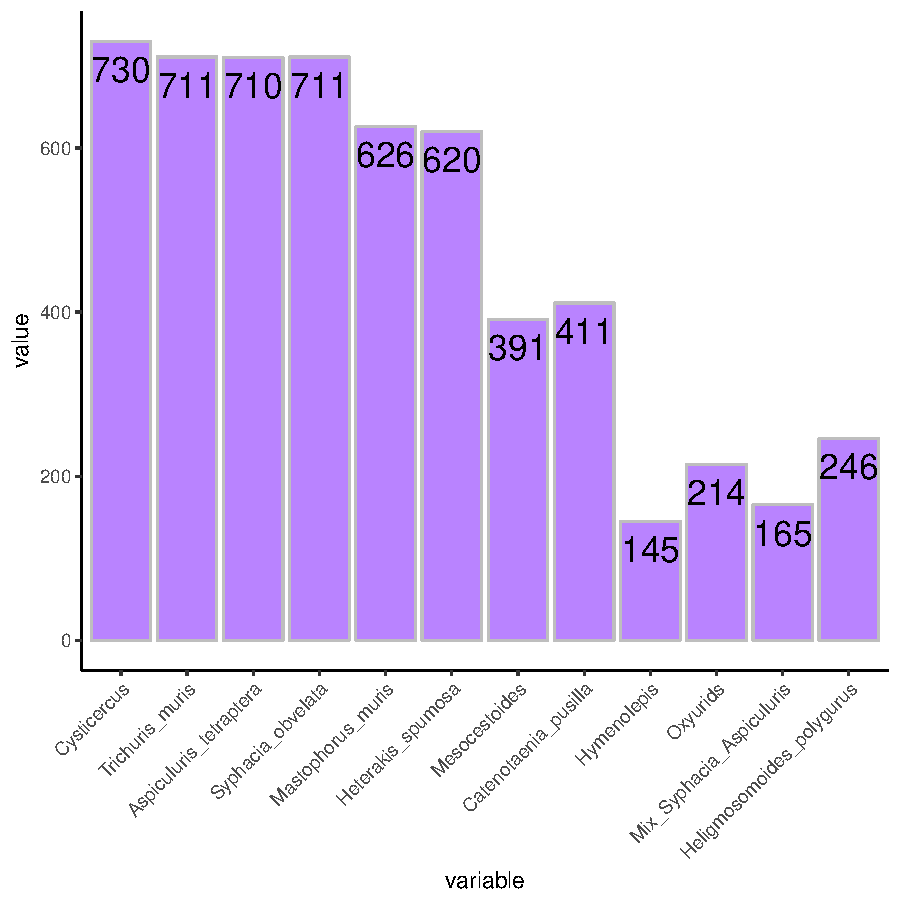
\includegraphics[width=.6\linewidth]{figure/Data-Analysis-Alice-2017-Rnwauto-report-13} 

}


\begin{kframe}\begin{alltt}
\hlcom{# prevalence at a locality depending on the density (only 2016, 2017)}

\hlstd{WormsDF2} \hlkwb{<-} \hlstd{TotalTable[}\hlkwd{c}\hlstd{(}\hlstr{"Cysticercus"}\hlstd{,} \hlstr{"Trichuris_muris"}\hlstd{,} \hlstr{"Aspiculuris_tetraptera"}\hlstd{,} \hlstr{"Syphacia_obvelata"}\hlstd{,}
                        \hlstr{"Mastophorus_muris"}\hlstd{,} \hlstr{"Heterakis_spumosa"}\hlstd{,} \hlstr{"Mesocestoides"}\hlstd{,}
                        \hlstr{"Catenotaenia_pusilla"}\hlstd{,} \hlstr{"Hymenolepis"}\hlstd{,} \hlstr{"Oxyurids"}\hlstd{,} \hlstr{"Mix_Syphacia_Aspiculuris"}\hlstd{,}
                        \hlstr{"Heligmosomoides_polygurus"}\hlstd{,} \hlstr{"Latitude"}\hlstd{,} \hlstr{"Longitude"}\hlstd{,} \hlstr{"density"}\hlstd{)]}

\hlstd{WormsDF2} \hlkwb{<-} \hlkwd{na.omit}\hlstd{(}\hlkwd{melt}\hlstd{(WormsDF2,} \hlkwc{id} \hlstd{=} \hlkwd{c}\hlstd{(}\hlstr{"Longitude"}\hlstd{,} \hlstr{"Latitude"}\hlstd{,} \hlstr{"density"}\hlstd{)))}

\hlstd{WormsDF2}\hlopt{$}\hlstd{prevalence} \hlkwb{<-} \hlnum{0}
\hlstd{WormsDF2}\hlopt{$}\hlstd{prevalence[WormsDF2}\hlopt{$}\hlstd{value} \hlopt{>} \hlnum{0}\hlstd{]} \hlkwb{<-} \hlnum{1}

\hlstd{aggworms2} \hlkwb{<-} \hlkwd{aggregate}\hlstd{(}\hlkwc{x} \hlstd{= WormsDF2[}\hlstr{"prevalence"}\hlstd{],}
          \hlkwc{by} \hlstd{= WormsDF2[}\hlkwd{c}\hlstd{(}\hlstr{"Latitude"}\hlstd{,} \hlstr{"Longitude"}\hlstd{,} \hlstr{"density"}\hlstd{,} \hlstr{"variable"}\hlstd{)],} \hlkwc{FUN} \hlstd{=} \hlkwa{function}\hlstd{(}\hlkwc{x}\hlstd{)\{}\hlkwd{sum}\hlstd{(x)}\hlopt{/}\hlkwd{length}\hlstd{(x)\})}

\hlkwd{ggplot}\hlstd{(}\hlkwc{data}\hlstd{=aggworms2,} \hlkwd{aes}\hlstd{(}\hlkwc{x} \hlstd{= density,} \hlkwc{y}\hlstd{=prevalence,} \hlkwc{col} \hlstd{= variable))} \hlopt{+}
  \hlkwd{geom_smooth}\hlstd{(}\hlkwc{alpha} \hlstd{=} \hlnum{0.1}\hlstd{,} \hlkwc{size} \hlstd{=} \hlnum{2}\hlstd{)} \hlopt{+}
  \hlkwd{geom_point}\hlstd{(}\hlkwc{col} \hlstd{=} \hlstr{"black"}\hlstd{)} \hlopt{+}
  \hlkwd{theme_classic}\hlstd{()}
\end{alltt}


{\ttfamily\noindent\itshape\color{messagecolor}{\#\# `geom\_smooth()` using method = 'loess' and formula 'y \textasciitilde{} x'}}\end{kframe}

{\centering 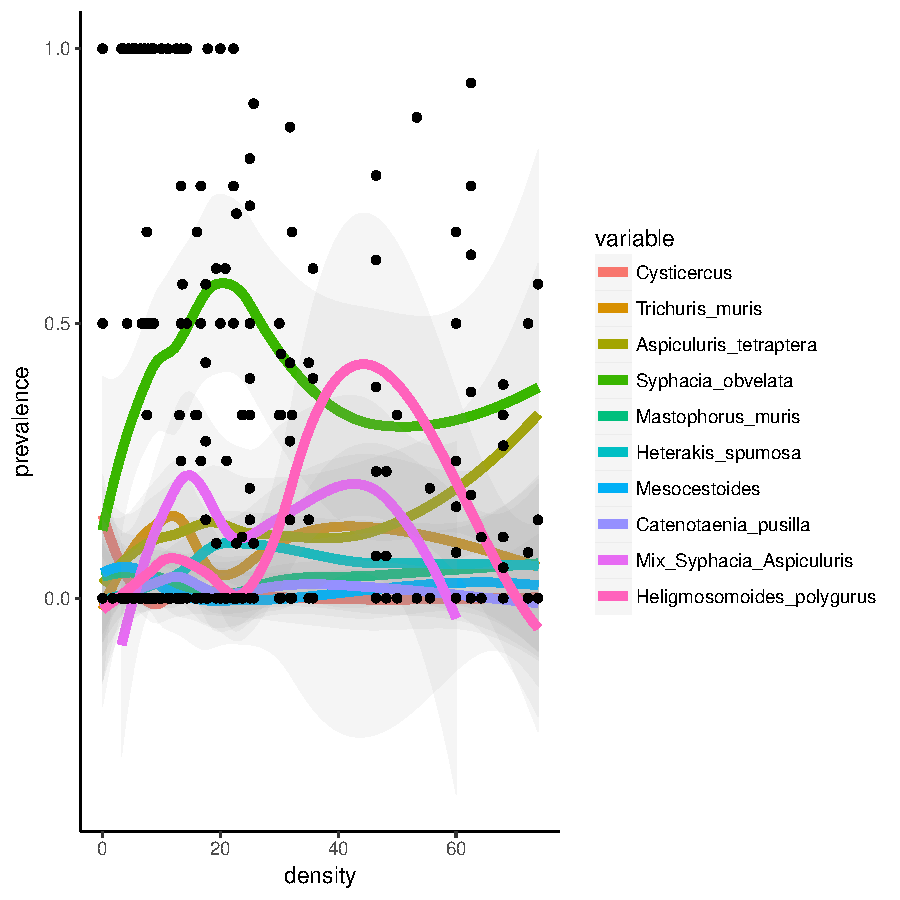
\includegraphics[width=.6\linewidth]{figure/Data-Analysis-Alice-2017-Rnwauto-report-14} 

}


\begin{kframe}\begin{alltt}
\hlcom{#***************************}
\hlcom{## To finish}

\hlcom{# link eimeria and prevalence }
\end{alltt}
\end{kframe}
\end{knitrout}

The R session information (including the OS info, R version and all
packages used):

\begin{knitrout}
\definecolor{shadecolor}{rgb}{0.969, 0.969, 0.969}\color{fgcolor}\begin{kframe}
\begin{alltt}
\hlkwd{sessionInfo}\hlstd{()}
\end{alltt}
\begin{verbatim}
## R version 3.3.3 (2017-03-06)
## Platform: x86_64-pc-linux-gnu (64-bit)
## Running under: Debian GNU/Linux 9 (stretch)
## 
## locale:
##  [1] LC_CTYPE=en_US.UTF-8       LC_NUMERIC=C               LC_TIME=en_US.UTF-8       
##  [4] LC_COLLATE=en_US.UTF-8     LC_MONETARY=en_US.UTF-8    LC_MESSAGES=en_US.UTF-8   
##  [7] LC_PAPER=en_US.UTF-8       LC_NAME=C                  LC_ADDRESS=C              
## [10] LC_TELEPHONE=C             LC_MEASUREMENT=en_US.UTF-8 LC_IDENTIFICATION=C       
## 
## attached base packages:
## [1] stats     graphics  grDevices utils     datasets  methods   base     
## 
## other attached packages:
## [1] knitr_1.15.1        ggrepel_0.6.5       GGally_1.3.2        devtools_1.13.3    
## [5] data.table_1.10.4-3 ggmap_2.6.1         ggplot2_2.2.1.9000 
## 
## loaded via a namespace (and not attached):
##  [1] Rcpp_0.12.13       highr_0.6          RColorBrewer_1.1-2 git2r_0.19.0      
##  [5] plyr_1.8.4         prettyunits_1.0.2  tools_3.3.3        progress_1.1.2    
##  [9] digest_0.6.12      evaluate_0.10      memoise_1.1.0      tibble_1.3.4      
## [13] gtable_0.2.0       lattice_0.20-34    png_0.1-7          rlang_0.1.4       
## [17] mapproj_1.2-5      curl_2.8.1         proto_1.0.0        withr_2.1.0.9000  
## [21] stringr_1.2.0      httr_1.2.1         RgoogleMaps_1.4.1  maps_3.2.0        
## [25] grid_3.3.3         reshape_0.8.7      R6_2.2.2           jpeg_0.1-8        
## [29] sp_1.2-4           reshape2_1.4.2     magrittr_1.5       MASS_7.3-45       
## [33] scales_0.5.0.9000  assertthat_0.1     geosphere_1.5-5    colorspace_1.3-2  
## [37] labeling_0.3       stringi_1.1.2      lazyeval_0.2.1     munsell_0.4.3     
## [41] rjson_0.2.15
\end{verbatim}
\begin{alltt}
\hlkwd{Sys.time}\hlstd{()}
\end{alltt}
\begin{verbatim}
## [1] "2017-11-20 19:09:03 CET"
\end{verbatim}
\end{kframe}
\end{knitrout}


\end{document}
